\documentclass[../main/main.tex]{subfiles}

\newdate{date}{19}{10}{2020}

% \begin{figure}[h!]
% \centering
% \includegraphics[page=6,width=0.8\textwidth]{../lessons/pdf_file/09_lecture.pdf}
% \end{figure}

%\displaydate{date}. Compiled:  \today. Alice.

\begin{document}

\pagestyle{plain}

\section{Lecture 9}


\subsubsection*{Slide 1}

\begin{minipage}[]{0.5\linewidth}
\centering
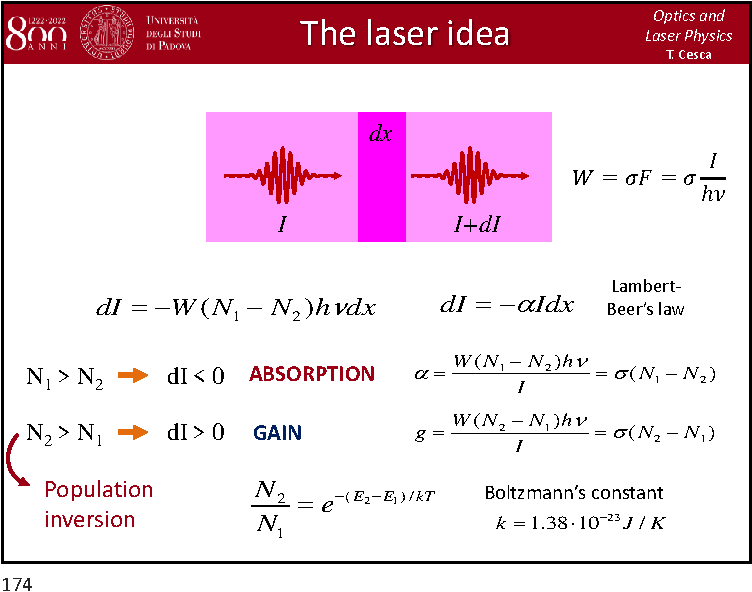
\includegraphics[page=1,width=1\textwidth]{../lessons/pdf_file/09_lecture.pdf}
\end{minipage}
\hspace{0.3cm}\vspace{0.3cm}
\begin{minipage}[c]{0.47\linewidth}

Let us consider an active material with thickness \( \dd[]{x}  \) and we shine a beam of intensity \( I \). We want to determine the intensity variation \( \dd[]{I}  \) after the beam is passed.

The first effects we have to consider is stimulated emission which produce photons and the second effect is absorption which remove photons:
\begin{equation*}
  \dd[]{I} = - W ( \mathcolorbox{green!20}{N_1} - \mathcolorbox{yellow!40}{N_2}) h \nu \dd[]{x}
\end{equation*}
the green term is the absorption term, the yellow is the stimulated emission phenomenum (add photon to the total).
We can rewrite the same expression with the \textbf{Lambert-Beer's law} (which relate to the \textbf{absorption coefficient}).

\end{minipage}

The \textbf{absorption} coefficient is related to the cross section for stimulated emission (or absorption since they are the same for non degenerate levels) multiplied by the difference \( N_1 - N_2 \).

The opposite situation is when \( N_2 > N_1 \), we have a net balance which is positive. That means that we have a net \textbf{gain}, we increase the number of photons inside the medium (opposite of the absorption coefficient).

The condition \( N_2 > N_1 \) is not an equilibrium one. At equilibrium, \( N_1 \) and \( N_2 \) are related to Boltzmann statistic which said us that we have always \( N_1 > N_2 \) (we can have only absorption). To get gain, we have to do \textbf{population inversion} with a pumping system which lead the system to an out-of-equilibrium condition.

\subsubsection*{Slide 2}

\begin{minipage}[]{0.5\linewidth}
\centering
\includegraphics[page=2,width=1\textwidth]{../lessons/pdf_file/09_lecture.pdf}
\end{minipage}
\hspace{0.3cm}\vspace{0.3cm}
\begin{minipage}[c]{0.47\linewidth}

Let us suppose that we obtained the condition of gain \( N_2 > N_1 \). We have a piece of material of length \( l \) and we insert it in an optical cavity. We consider the \textbf{Fabry-Perot cavity} which is formed by two mirrors one with reflectivity \( R_1 = 100 \% \) and the other with \( R_2 < 100 \% \) to extract the beam out of the cavity.

If we enter with a photon flux \( F_{in} \), at the output \( F_{out} \) we have an exponential increasing depending on the gain.

We want to determine the photon flux passing just one time through the system (one step forward and backward).

\end{minipage}

Just travelling inside the cavity we may lose photons (for instance a non perfect alignment). The factor \( (1-L_i) \) are the photons that remain in the cavity, so \( L_i \) are the losses. We arrive to the second mirror \( R_2 \), we pass to the medium again (we have again the exponential gain) and we lose again photons and we pass again on the first mirror \( R_1 \).
In this way, we can compute the photon flux at the end.

The \textbf{threshold} condition is that the photon flux at the end is the same of the beginning. This means that the gain is compensating exactly the photon that are lost due to reflection of the mirror or any other loss sources inside the cavity.

Assuming to be in the threshold condition, it is immediate to derive the formula for the \textbf{critical inversion}.

It can be written in a more compact form as:
\begin{equation*}
  N_c = \frac{\gamma  }{\sigma l}
\end{equation*}
where \( \gamma   \) are the \textbf{logarithmic cavity losses per single pass}. This is a difference of the population at 1 and 2.

\subsubsection*{Slide 3}

\begin{minipage}[]{0.5\linewidth}
\centering
\includegraphics[page=3,width=1\textwidth]{../lessons/pdf_file/09_lecture.pdf}
\end{minipage}
\hspace{0.3cm}\vspace{0.3cm}
\begin{minipage}[c]{0.47\linewidth}

The key point is to have the \textbf{population inversion}, i.e. an increasing in intensity. How is it possible to get it?
Pumping is necessary to populate the high energy level.

Let us consider a material in which the important transition are the one between these \textbf{two levels}. We pump from 1 to 2, and we have transition from 2 to 1.
In this condition, it is easy to obtain that at most we obtain the balance \( N_2 = N_1 \). The variation of intensity will go to zero as soon \( N_2 = N_1 \) and the material become transparent to radiation. You cannot pump it anymore, you will not produce any effect.

For this purpose, we need to have a system in which we need to consider more than two levels!

\end{minipage}

Let us consider a \textbf{three level system}. We gain a lower energy level 1 and an upper energy level 2. Moreover, we have a energy level 3 above 2.
We have a pump that occur from 1 to 3. From the 3 level, the system is able to decay rapidly to 2. Typically, we want that this decay is non radiative (we want that it occur in a very fast way and it does not emit photon).

In this ideal case, if we consider that the total population is \( N_t = N_1 + N_2 + N_3 \), it is easy to see that to obtain inversion of the population we need to overcome half the total population: \( N_2 > N_t /2 \). We can think that if the decay from 3 to 2 is fast, we can suppose that the population \( N_3 = 0 \) always.

This is a little more difficult, because there is a treshold, we need \( N_2 \) above the value \( N_t/2 \).

In particular, it is more difficult wrt to a \textbf{four level system}.
We pump from 1 to 4. We want that the decay from 4 to 3 occurs very fast. Then, we have the laser transition. After that, we have the decay from 2 to 1 which is very fast such that it could be considered empty.

If 2 is always empty, it means that as soon as we have an atom in 3 we can get population inversion because we have always \( N_2>N_1 \) and we do not have a treshold anymore!

\subsubsection*{Slide 4}

\begin{minipage}[]{0.5\linewidth}
\centering
\includegraphics[page=4,width=1\textwidth]{../lessons/pdf_file/09_lecture.pdf}
\end{minipage}
\hspace{0.3cm}\vspace{0.3cm}
\begin{minipage}[c]{0.47\linewidth}

The most important example of a three level system is the \textbf{Ruby laser}.

\end{minipage}

\subsubsection*{Slide 5}

\begin{minipage}[]{0.5\linewidth}
\centering
\includegraphics[page=5,width=1\textwidth]{../lessons/pdf_file/09_lecture.pdf}
\end{minipage}
\hspace{0.3cm}\vspace{0.3cm}
\begin{minipage}[c]{0.47\linewidth}

This is an example of a four level system: \textbf{Nd:YAG laser}.

\end{minipage}

\subsubsection*{Slide 6}

\begin{minipage}[]{0.5\linewidth}
\centering
\includegraphics[page=6,width=1\textwidth]{../lessons/pdf_file/09_lecture.pdf}
\end{minipage}
\hspace{0.3cm}\vspace{0.3cm}
\begin{minipage}[c]{0.47\linewidth}

The laser transition occur between two levels with a given frequency. In reality, it never happens that the transition is so sharp that we have a dirac delta in term of frequency but we have a \textbf{line broadening}. We have to consider a \textbf{bandwidth}.

We will distinguish two mechanism which can produce broadening:

\begin{itemize}
\item \textbf{homoegeneous broadening}.
\item \textbf{inhomogeneous broadening}.
\end{itemize}

In \textbf{homoegeneous broadening} we consider all the atoms within the material equal. The most simple mechanism is what is called \textbf{collisional broadening}.

\end{minipage}

Let us suppose to have a gas an active medium, we have the collisions among the atoms which are related to the pressure inside the chamber. In this case, all the atoms can be seen as equal. This collisions induce a broad of the line which can be described by a \textbf{Lorentzian} curve.

\( \tau _c \) is the average time between two collisions.

We can see the comparison between the homoegeneous broadening between the three types of laser.

Having a large bandwidth can make a difference. Different methods for having laser working in different ways can be applied to some laser and not to others according to the linewidth of the system. That is why it is important to remember these numbers

\subsubsection*{Slide 7}

\begin{minipage}[]{0.5\linewidth}
\centering
\includegraphics[page=7,width=1\textwidth]{../lessons/pdf_file/09_lecture.pdf}
\end{minipage}
\hspace{0.3cm}\vspace{0.3cm}
\begin{minipage}[c]{0.47\linewidth}

The \textbf{natural broadening} is a broadening that you cannot avoid which is not related to the temperature (you can decrease the temperature but nothing change). It is instead related to the fact that the lifetime for a spontaneous emission for a level is always finite! This would be zero only for an infinite lifetime \( \tau _{sp} \).

It is like considering the uncertanty principle in terms of energy and time. Given a \( \Delta t \), you have uncertanty on energy (or on frequency).

\end{minipage}

\subsubsection*{Slide 8}

\begin{minipage}[]{0.5\linewidth}
\centering
\includegraphics[page=8,width=1\textwidth]{../lessons/pdf_file/09_lecture.pdf}
\end{minipage}
\hspace{0.3cm}\vspace{0.3cm}
\begin{minipage}[c]{0.47\linewidth}

The \textbf{inhomogeneous broadening} appears every time you can distinguish the atoms in your material according to how they broaden the lineshape.

The material is composed by a set of atoms and for each set you have an homoegeneous broadening. But you have a convolution of these homoegeneous broadened lineshape, which produce an inhomogeneous lineshape. It can be modeled by a \textbf{Gaussian} (or \textbf{Doppler} brodening).

Let us consider a gas, we a Brownian motion of the atoms and we send a beam. From the point of view of the beam, we have atoms moving in all directions and so for the Doppler effect, the atoms feel different frequency according to the velocity and direction they are moving. You see the transition of each atoms slighly different in frequency.

\end{minipage}

In an He-Ne laser the inhomogeneous broadening is dominating wrt the homoegeneous processes.

This effect can be present also in solid-state lasers (altough you do not have atoms moving). The crystal field can be different due to the presence of defects. If the local field is different, you can have a \textbf{Stark effect} which produce a difference in energy that you have to consider between the levels.

In many case, particularly for the solid-state laser, the homoegeneous broadening is the dominant effect. For gas lasers, inhomogeneous broadening is a source of broadening.


\subsubsection*{Slide 9}

\begin{minipage}[]{0.5\linewidth}
\centering
\includegraphics[page=9,width=1\textwidth]{../lessons/pdf_file/09_lecture.pdf}
\includegraphics[page=10,width=1\textwidth]{../lessons/pdf_file/09_lecture.pdf}
\end{minipage}
\hspace{0.3cm}\vspace{0.3cm}
\begin{minipage}[c]{0.47\linewidth}

Comparison of the shape of the two types of broadening. You can determine what is the dominant effect by fitting and seeing if the curve is a Lorentzian or a Gaussian.

Any time that we have inhomogeneous drawing, we can always think this as the convolution of homoegeneous broadening (plot on the right). 

\end{minipage}




\end{document}
